\documentclass{article}\usepackage[]{graphicx}\usepackage[]{color}
% maxwidth is the original width if it is less than linewidth
% otherwise use linewidth (to make sure the graphics do not exceed the margin)
\makeatletter
\def\maxwidth{ %
  \ifdim\Gin@nat@width>\linewidth
    \linewidth
  \else
    \Gin@nat@width
  \fi
}
\makeatother

\definecolor{fgcolor}{rgb}{0.345, 0.345, 0.345}
\newcommand{\hlnum}[1]{\textcolor[rgb]{0.686,0.059,0.569}{#1}}%
\newcommand{\hlstr}[1]{\textcolor[rgb]{0.192,0.494,0.8}{#1}}%
\newcommand{\hlcom}[1]{\textcolor[rgb]{0.678,0.584,0.686}{\textit{#1}}}%
\newcommand{\hlopt}[1]{\textcolor[rgb]{0,0,0}{#1}}%
\newcommand{\hlstd}[1]{\textcolor[rgb]{0.345,0.345,0.345}{#1}}%
\newcommand{\hlkwa}[1]{\textcolor[rgb]{0.161,0.373,0.58}{\textbf{#1}}}%
\newcommand{\hlkwb}[1]{\textcolor[rgb]{0.69,0.353,0.396}{#1}}%
\newcommand{\hlkwc}[1]{\textcolor[rgb]{0.333,0.667,0.333}{#1}}%
\newcommand{\hlkwd}[1]{\textcolor[rgb]{0.737,0.353,0.396}{\textbf{#1}}}%
\let\hlipl\hlkwb

\usepackage{framed}
\makeatletter
\newenvironment{kframe}{%
 \def\at@end@of@kframe{}%
 \ifinner\ifhmode%
  \def\at@end@of@kframe{\end{minipage}}%
  \begin{minipage}{\columnwidth}%
 \fi\fi%
 \def\FrameCommand##1{\hskip\@totalleftmargin \hskip-\fboxsep
 \colorbox{shadecolor}{##1}\hskip-\fboxsep
     % There is no \\@totalrightmargin, so:
     \hskip-\linewidth \hskip-\@totalleftmargin \hskip\columnwidth}%
 \MakeFramed {\advance\hsize-\width
   \@totalleftmargin\z@ \linewidth\hsize
   \@setminipage}}%
 {\par\unskip\endMakeFramed%
 \at@end@of@kframe}
\makeatother

\definecolor{shadecolor}{rgb}{.97, .97, .97}
\definecolor{messagecolor}{rgb}{0, 0, 0}
\definecolor{warningcolor}{rgb}{1, 0, 1}
\definecolor{errorcolor}{rgb}{1, 0, 0}
\newenvironment{knitrout}{}{} % an empty environment to be redefined in TeX

\usepackage{alltt}
\usepackage{graphicx}
\usepackage{tabularx}
\usepackage{natbib}


\usepackage{array}
\usepackage{amsmath}
%\usepackage[backend=bibtex]{biblatex}
\setkeys{Gin}{width=0.8\textwidth}
%\setlength{\captionmargin}{30pt}
\setlength{\abovecaptionskip}{10pt}
\setlength{\belowcaptionskip}{10pt}
 \topmargin -1.5cm 
 \oddsidemargin -0.04cm 
 \evensidemargin -0.04cm 
 \textwidth 16.59cm
 \textheight 21.94cm 
 \parskip 7.2pt 
\renewcommand{\baselinestretch}{1.2} 	
\parindent 0pt

\bibliographystyle{..//..//refs/bibstyles/amnat.bst}
\usepackage{xr-hyper}
\usepackage{hyperref}
\title{Competition between native \textit{Cryptotaenia canadensis} and invasive \textit{Hesperis matronalis} seedlings is mediated by relative germination timing}
\IfFileExists{upquote.sty}{\usepackage{upquote}}{}
\begin{document}
\maketitle
Invasive plants are often characterized by rapid germination and precocious phenology (the timing seasonal life cycle events ) \citep{wolkovich, and other, and other}. Rapid phenology may server as a seasonal or short term priorty effect, confering a competitive advantage by allowing species to begin drawing down seasonal resources and modifying their environment before their competitors emerge \citep{}. Rapid germination and phenology

\section{Introduction}
\textbf{A core task of invasion biology it to identify trait that make a species likely do be invasive}
\begin{enumerate}
\item Invasive species are characterized by rapid germination and precocious phenology
\item Being so early may function as a seasonal priority effect-niche premption and such
\item This seasonal priority effect might contribute to the competitive dominacne and invasion success of invasives
\end{enumerate}

\textbf{But it is difficult to infer mechanism from observational studies}
\begin{enumerate}
\item Because rapid phenology often covaries with other competitive traits. You'd need super high resolution phenolgy and climate data.
\end{enumerate}

\textbf{Experiments can test role of SPE's in plant competition}
\begin{enumerate}
\item  A common approach is to use sequential planting studies.
\item recent review paper on these experiments by \citet{Weidlich:2020aa}: 42\% of such studies included planting interval treatments of less than 1 month, approximating the time scale of SPEs and all found evidence of priority effects. (How many were invasive vs. native?)
\end{enumerate}

\textbf{Yet the extent to which these studies are generailizable is questionable}
\begin{enumerate}
\item  Almost all mechanistic tests for SPEs to date have been performed using species from temperate grasslands \citep{Weidlich:2020aa}, whose germination behavior may differ substantially from taxa in other habitats \citep{Tudela-Isanta:2018aa}.
\item In many ecosystems, plant communities must re-assemble each year after a period of dormancy. In these communities, priority effects are largely the product of the rate at which dormant plants and seeds respond to their environment and resume growth or germinate when favorable conditions return \citep{Rudolf:2019aa}, rather than the the timing of the arrival of propagules, which in many cases occurs prior to the dormant season \citep{Howe:1982aa,Baskin:1988aa}.
\item Therefore, sequential plantings cannot address how important SPE's are in nature because the priority effect is 100\% contigent on the choice of the treatment.
\end{enumerate}

\textbf{In ecological systems where dormancy is common like temperate  and boreal forest, say a few other here, environmental conditions such as temperature (cold stratification and incubate), soil moisture, and light control the release of dormancy and germination or growth.}
\begin{enumerate}
\item Cohabiting species respond with different sensitivites to these elements; and this may be especially true for invasive species which evolved under different climate condition in their home vs. invaded ranges.
\item And climate elements vary over time
\item Together, this suggests that germination or phenological responses between competing species will converge and divirge periodically over time, depending the their specific sensitives and the climate they experience.
\item This variation can be leverage for mechanistic tests of SPEs by a) qunatify how the phenoligical lag between species changes under realistic climate variation , and b) the effect of this variation on competition
\end{enumerate}

\textbf{Leveraging natural climate variation to test SPEs has major beneifits}
\begin{enumerate}
\item SPE's are a cornerstone of community assembly theory and modern coexistence theory, and mechansitically qunatifying their contribtion in community interactions is important
\item Anthropogenic climatic change is altering the  environments \citep{Walck2011} and changing  germination and phenology patterns. Such sustained alterations to environmental cues have potential to disrupt SPEs, shifting balances of species' interactions, changing patterns of invasion, and strongly influence biological filtering of communities..
\item So assessing the role of SPE's in species interactions under more realistic germination environments is timely because it can be used to improve spatio-temporal predictions of species interaction under novel climate conditions.
\end{enumerate}

\textbf{While invasibility, competion, coexistance etc is a property of individual and community interactions, pair-wise comparisons have been a useful tool to identifying and quatify mechanisms of species interactions}
\begin{enumerate}
\item Why am I saying this? Probably to justify the limited taxonomic scope of my study
\end{enumerate}

\textbf{Using a combination of germination assays, competition trials and climate projections, we:}
\begin{enumerate}
\item Quantify gernmination behavior of varying environments to estimate a realistic range of climate driven priority between an widespread invasive and native forb species. 
\item Compete them to assess the influences of priority effect on competitive outcome and quantify SPE's contribution vs. other intrinsic competition traits.
\item Use relationship between climate and germination behavior to make first-pass, quick and dirtay and rough prediction about where where interactions between these two species may shift with climate change as a proof-of-concept case study to build on in the future.
\end{enumerate}

\section*{Methods}
\subsection{Focal species}
 Dames Rocket (\textit{Hesperis matronalis}) is a herbaceous biennial/perennial species originally from Eurasia, and introduced to North America in the 19th century \citep{Francis} It  can rapidly invade  meadows, forest edges and woodland, forming dense, monotypic stands and excluding native vegetation \citep{}. It is currently listed as a noxious or invasive weed is several states and provinces in the United States and Canada. Honewort (\textit{Cryptotania canadensis}) is a herbaceous perennial in the \textit{Apiaceae} family, native to forests and woodland of North America. The  habitat overlap of these two species suggests that they may compete in nature. While their apparent niche may be similar, the two species display a substantial different germination niche, making them a suitable model for our study. \textit{C. canadensis} seeds are classified with non-deep physiological dormancy and require a substantial  period of cold moist stratification to release dormancy and initiate germination. While some reports suggests that cold stratification enhances germination in \textit{H. matronalis} at low incubation temperatures \citep{} several studies have demonstrated that this fresh and after-ripened (dry-stored) seeds of \textit{H. matronalis} are capable of rapid and complete germination at average spring temperatures in the temperate zone \citep{}. The dynamics suggest that the phenolgical differences in germination among the species have potential to be strong mediated by cold stratification and incubation.  

\subsection{Germination Assays}
To investigate the relationship between environmental variation and relative germination timing between our two focal species, we obtained seeds of \textit{C. canadensis} from Prairie Moon Nursery (Winona, MN) and seed of \textit{H. matronalis} from American Meadows (Shelburne, VT). We performed germination assays in the growth facilities of Arnold Arboretum in Boston MA (42.3074\degree N, 71.1208\degree W). We assigned seeds to a fully crossed set of twenty experimental treatments; 10 levels of of cold stratification duration (0,14,28,35,42,49,56,63,77,91 days at 4\degree C) , two levels of incubation temperature (warm--- 25\degree C:15\degree C (day/night), cool--- 20\degree C:10\degree C (day/night)).

\noindent  Prior to applying experimental treatments we applied a ``float test" in which all seeds were placed in distilled water and unfilled seeds (floating) were removed from the experiment \citep{Baskin2014}. The remaining seeds were imbibed in distilled water for 24 hours after which we placed 20 seeds per species/ treatment combination in petri dish on moist pool filter sand. We replicated each treatment combination three times. For the cold stratification treatments, we wrapped petri dishes in aluminum foil to prevent light exposure and placed them in a growth chamber at 4\degree C. After each stratification interval, we transferred the petri dishes to their assigned incubation chamber for 25 days, moistening the germination substrate as necessary to maintain maximum saturation of the medium without flooding the seeds. We check for new germinates every 2 days, defining a seed as germinated when its radical or cotyledon tissue was visable\citep{Baskin2014}. We assessed the viability of any seeds that did not germinate in the 25 day incubation trial by performing a ``crush test" in which we applied pressure to the intact seed to evaluate its condition \citep{Baskin2014}. We excluded any subsequent seeds deemed deemed unviable from all subsequent analyses. Due to the staggering of our stratification treatments the experiment took place between 27 August- 12 December 2018.\\

\subsubsection*{Statistical analysis}
To assess interspecific differences in the relationship between germination rate and temperature variability, In addition to reporting descriptive statistics for each treatment (maximum germination, mean germination time). we fit a Bayesian mixed-effect accelerated failure time model (AFT) with weeks of stratification and incubation temperature and species as fixed effects.  We chose an AFT model as it allowed for us to account for viable seeds that did not germinate during our incubation window letting us robustly compare germination timing (t50 time to 50\% germination) even among treatments with different final germination percentages in the time of the experiment\citep{Soltani:2015aa}. One drawback of this approach is that these classes models assume that all viable seeds will eventually germination, an assumption which we would not expect to be true in nature. For this reason, we considered any estimate t50 values greater than 60 days to suggest that particular seed lot would not reach 50\% germination under those conditions.\\ %%woof say better.

\noindent We fit the model using the R package ``brms" \citep{Burkner2018} using a weibull distribution for the model's likelihood function. We ran the model on four chains with 4000 iterations and a 3000 iteration warm up for a total of 4000 posterior draws for each parameter using weakly informative priors. We assessed  model performance through ensuring $\hat{R}$s were between 1 and 1.01 and bulk and tail effective sample sizes were high.

\subsection{Competition Trials}
To quantify the contribution of SPEs to inter-specific competition dynamics, we chose two species from our germination trial \textit{Cryptotaenia canadensis} and \textit{Hesperis matronalis} for competition trials. We chose these species because the germination of \textit{C. candensis} advanced strongly with increasing cold stratification, while seeds of \textit{H. matronalis} germinated rapidly under all conditions suggesting that under low stratification treatments there would be a strong priority effect between the species that would diminish as stratification time increased. Additionally \texit{H. matronilis},originally from Eurasia, is considered an invasive species or noxious weed in many parts of North America and so evaluating the role of SPE's in this species's competitive ability has potential applied benefits for the management of this species.\\

\noindent Competition trials took place under controlled condition in a research greenhouse at the Arnold Arboretum in October 2020-February 2021. We planted seeds into 3.5 in square pots, employing a response surface design where we varied both the overall density of seeds and proportion of each species in each pot \citep{Inouye2001}. High and low density treatments consisted of 14 and 8 seeds respectively. Our proportion treatments (100:0\%. 25:75\%, 50:50\%, 75:25\%, 0:100\% (species A :species B)) Each density by proportion treatment was replicated six times. This design allows us to evaluate effects of inter- and intra- specific competion and density dependence independently and in association with our experimental treatment.\\

\noindent To test the effects of temporal priority on plant growth, we randomly assigned half of the pots low (45 days) and high (72 days) cold stratification treatments at 4\degree C. We staggered the start of the treatments, so that at the conclusion of the pre-treatment, all pots were transferred to a heated greenhouse maintained at 15-25 \degree C with 14 hours of supplemental light. Germination was observed daily from 24 December- Jan 13 and every two days from 15 Jan to 1 Feb. The locations of each pot in the greenhouse were randomly reassigned every 3 days to minimize any blocking effects on germination or growth.

\noident After 35 days, we added 1 tsp per 1 gallon of water of Peter’s 20-10-20 liquid feed fertilizer to all pots. After 62 days, we harvested the above group biomass from all pots, dried them in a oven for 48 hours at 60\degree C, and recorded the dry weight of each species/pot using a Mettler balance.\\

\subsubsection*{Statiscal analysis}
\noindent We quantified the temporal priority between the species by subtracting the mean germination time (MGT) of \textit{H. matronalis} from that of \textit{C. canadensis} in each pot. This allowed us to apply priority treatment as a regression design \citep{} with priority levels ranging from -1.3 to 9.5 (\textit{C. candensis} mean germination time 1.3 days earlier to 9.5 days later than that of \textit{matronalis}).\\

\noindent We assessed the impact of competitor density and relative germination timing on species biomass with two different frameworks.

First we calculated the average per-capita biomass of each species per pot, by divided each species' plot level biomass by its number of germinants. We then set up a system of pair-wise equations in which the per-capita biomass of each species was regressed against the density of conspecific seeds, density of competitor seeds, and the difference in mean germination time among them using Bayesian linear models. The equation is written below.

\begin{align*}

biomass_{C. canadensis}  &= \alpha +& \beta_{1}*density_{C. canadensis} + \beta_{2}*density_{H. matronalis}+\beta_{3}*$\delta$MGT + \epsilon} 

biomass_{H. matronalis}  &= \alpha +& \beta_{1}*density_{C. canadensis} + \beta_{2}*density_{H. matronalis}+\beta_{3}*$\delta$MGT + \epsilon}

\end{align*}


In the formulation, the $beta$_1$ is the estimated effect of intra-specific competition, $beta_2$ is the estimated effect of inter-specific competition, and $beta_3$ is the estimated priority effect. From these estimates we calculated the competition coefficients (c) (ratio of intra- to inter-specific competition strength) for each species, with and without the additive effects of germination phenology differences.

\begin{align*}

c_{sp1}= b_1/b_2 

c_{with priority}= (b_1+b_3)/b_2

\end{align*}

We also assessed difference in biomass among density and phenology treatments by calculating the relative growth rate differences among species at the plot level . Like th per capita methods described above, this metric can be used to quantify the effects of initial species’ abundance, species identity and the environment on competition outcomes, but is designed to evaluate biomass composition at the community level \citep{Connolly2005}.

For each plot, we calculated the relative growth rate difference among species using the equation below developed by \citet{Connolly2005}.
We then modeled the effect of seed density of \textit{C. canadensis}, \textit{H. matronalis} and $\delta$ mean germination time using Bayesian linear regression.

Both models were run using the R packages ``brms'' using weakly informative prior. We ran all models of 4 chains, with a 400 iterations per chain and a warm up of 3000 interations, for a total of 4,000 posterior samples per parameter. 



%\subsection*{Focal species}
%\subsection*{Germination Assays}
%\subsection*{Competition Trials}
%\subsection*{Data analysis}
%\textbf{Some thoughts on Connolleys RGRD models}
%\begin{enumerate}
%\item Data at the plot level which makes large assays like the one I did tractable compared with spatially explict ones like heygi index or neighborhood
%\item Also is desinged for signle season dynamics unlike Lotke-Volterra and the usual
%\item Weakness, isn't designed for monoculture treatments( which we explictely put in out study ) since you an't have the log of zero. Maybe I overcome this by %converting 0s to 00000.1

%\end{enumerate}
\section*{Results}
\subsection*{Relative germination phenology}
In our germination assays, \textit{H. matronalis} reach 50\% germination in under five days for all environmental treatments, always exceeded 85\% germination regardless of environmental conditions (Fig. \ref{}). Increasing cold stratification duration and incubation temperature only marginally only enhanced the germination rate of this species (Fig. \ref{}). By contrast, increasing incubation temperature had a negative effect of the germination rate of \textit{C. canadensis}, suggesting that the mean 20\degree C temperatures of our warm incubation treatment are supra-optimal for the species (Fig. \ref{}). Without sufficient cold stratification (>5 weeks for low incubation and > 7 weeks for high incubation temperatures), seeds of  \textit{C. canadensis} did not reach 50\% germination during the duration of our experiment (Fig. \ref{}). However, under high levels of cold stratification, (>7 weeks with cool incubation) germination rates of \textit{C.canadensis} began to converge on those of \textit{H. matronialis}, and at levels of stratification greater than 10-12 weeks and low incubation temperatures, the germination rate and fraction of \textit{C.canadensis} was well matched to that of \textit{H. matronalis} (Fig. \ref{}).

\subsection*{Effects of relative germination phenology on compeition}

\section*{Discussion}
\subsection*{Germination as a seasonal priority effect} 
In this study, we found that climate driven differences in the germination timing among species has strong impacts on their competitive dynamics. Our results join a growing body of experiments demonstrating that relative germination phenology can function as a seasonal or short term priority effect, enhancing the performance of the earliest germinating species at the expense of later germinants \citep{}. While this effect has been primarily commonly demonstrated in experiments in which the planting of competing seeds is staggered at increasing intervals \citep{}, we were able to generate substantial variation in relative germination timing among our competing species though by opporationalizing their differential sensitivity to environmental cues. 

In our germination assays, The germination behavior of \texit{H. matronalis} was little affected by cold stratification, while germination rate and speed of \texit{C. canadensis} was strongly enhanced with cold stratification, especially when germianted at cooler temperatures (Fig. \ref{fig:aft}). These differences are themselves not surprising as \textit{H. matronalis} seeds are considered non-dormant \citep{}, and seeds of \textit{C. canadensis} are physiologically dormant \citep{}. , These different responses generated germination dynamics in which under alternative low stratification regimes \textit{H. matronalis} cohorts germinated as much as two weeks before \textit{C. canadensis}, while under high stratification, the species germinated at approximately the same time (Fig. \ref{fig:aft}). 

In our competition trials, we observed that differences in germination on the order of a few days had substantial impacts on both the per capita and plot level relative growth rate differences among species (Fig \ref{fig:Cc},\ref{fig:RGRD}). If we consider the range of variability we observed (approximately two weeks lag to simultaneously)

These inter-specific dynamics we observed are comparable to treatments applied in staggered planting experiments \citep{}, but the fact that we were able to induce these effects through varying the germination environment rather than directly manipulating germination itself is an important phase for translating the estimates from priority effect experiments into natural systems.  suggests that the kinds of seasonal priority effects may be important for realz, especially in seasonal environments with high levels of inte-rannual climate variations.


\subsection*{Considering the impacts of seasonal priority effects in forest communities}
While most studies on seasonal priority effects focus on grassland environments with annual taxa \citep{} we explicitly conducted our experiment with forest perennials to better understand the generality of these effects to other ecological systems. While we found priority effects impacted within year dynamics of seedlings, our experiment was not designed to the longevity of these priority effects on the longer term dynamics of our focal species.  Many studies suggest that these short term priority effects many be transient, though several studies that used staggered planting methods at similar scale to the phenological lags we observed in our trials saw the influence of these initial priority effect on community composition several seasons later \citep{}. In perennial communities, these long terms dynamics are even more difficult to assess.

While it is well established that plants are must vulnerable to completion early in their lives.but\\
Ramets\\
Our study did not have a cost.
\\
Yet, even with this important step towards biological realism, more research is needed to understand the importance of germination priority effects, especially among perennial plants in seasonal environments.


Our experiment was designed to capture the dynamics on seedling competition, and we  (Mash up below paragraph into this one)

. Yet, by choosing these more complicated life forms, speculating on the long term impact of germination seasonal priority effects becomes further complicated. \textit{C. canadensis} can rely heavily on vegetative reproduction, clonal plants, competition among ramets may be a strong ecological determinant than competition among seedlings \citep{}. \textit{C. canadensis} also forms a transient seed bank \citep{}, suggesting that the within year dynamics of germination and growth captured in our study, could be decoupled from the among year dynamics. It also also invasives invade communities not population, two species studies are limited to predict the invasion dynamics of a species in real tim. No cost do being early.Cite Wainwright.

With these limitations, our study was not designed to predict the the long term dynamics of \textit{C. canadensis} and \textit{H. matronalis} underfield condtions. 

.This stage is super critical in general, talk about germination niche.
and we cannot assess the longevity of these priority effect, or their ulitmate impacts on fitness. We focused on species with complicated life histories and dynamics, seed banks, vegetative repro etc. 
With that it suggest our most relevant to the plant establishment, which is relevent both in the context of plant migration, disturbance, and ecological resotoration.

 

\subsection*{Phenological Diversity as a metric of something low-level jargony}
Our pairwise competition study indicates the phenological differences in germination time can strongly influence competitive outcomes. While empirical work with more species will help, if phenology is a mechanism of competitive domianence and invasion, it can also be a mechanisms of invasion resistance or co-existance. Read a bit about the invasability literature and suggest considering phenological diversity as a metri for assessing communities may be critical. COmparing across phases and life forms. Ie germinating seeds also competed with adults. This could be particular important for design ecological restorations. 

. Phenolgoical diversity. This will become more imporant with cliamte hcange as new temporal niches are created.
\subsection*{From germination requirements to germnation responses}
The first stage to incorperating phenological diversity


\textbf{So many caveats:}
\begin{enumerate}
\item These species are perennials, seeds banks. Given our expermental constrait couldn't account for these dynamics. ie competition my happen between raments and seeds. Our simplifed experimental design doesn't address these important factors, however they add an important piece to the puzzle. 
\item Given above, our results may be most relevant in colonization dynamics, especially in super disturbed systems where seed ins important.
\item Limitations of RGRD models from paper
\item We know invasives invade communities not population, two species studies are limited to predict the invasion dynamics of a species in real time
\item What we did do was quantify the contribution of priority effect to invasion success. It's high. This suggest restorations could benefit from consider phenological diversity 
\end{enumerate}

\begin{figure}[h!]
    \centering
         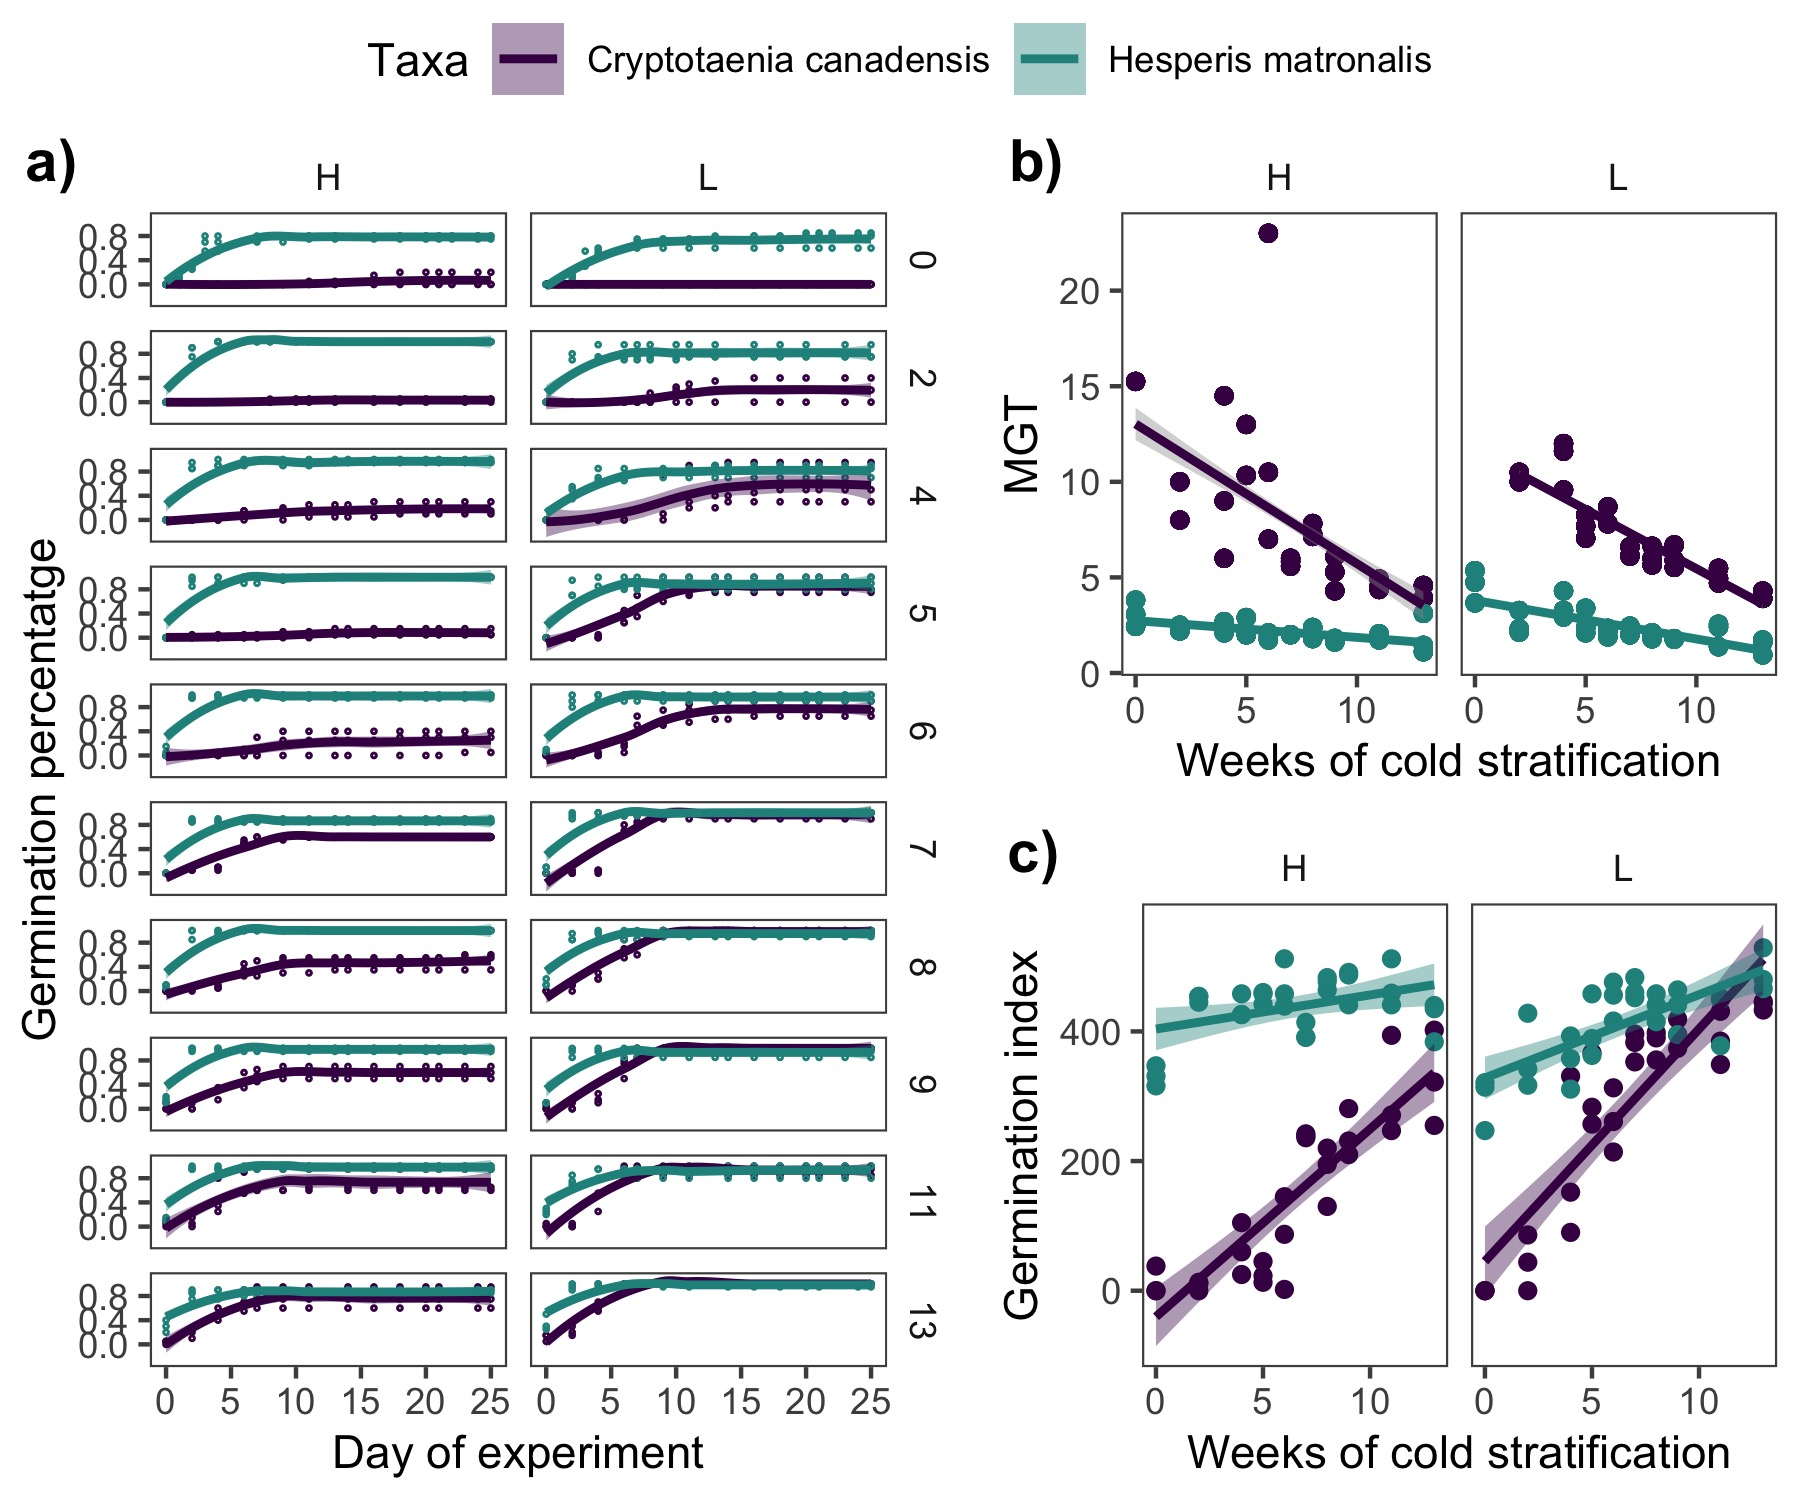
\includegraphics[width=\textwidth]{..//figure/crp_hesp1.jpeg}
    \caption{Germination behavior of \textit{H. matronalis} and \texit{C. canadensis} indicate that the rate of \texit{C. canadensis} approaches that of \textit{H. matronalis} under cool temperatures and high levels of stratification. a) Shows germination time courses for both species at each level of incubation (H,L) and stratitification (0-13, y-axis). b) Dipicts Mean germination time for each species as a function of weeks of stratifcation and both high (H) and low (L) incubation temperature. c) Show a composite germination index for each species that account for the speed and percentage of germination for each species as a function of weeks of stratifcation and both high (H) and low (L) incubation temperature. } 
    \label{fig:aft}
\end{figure}

\begin{figure}[h!]
    \centering
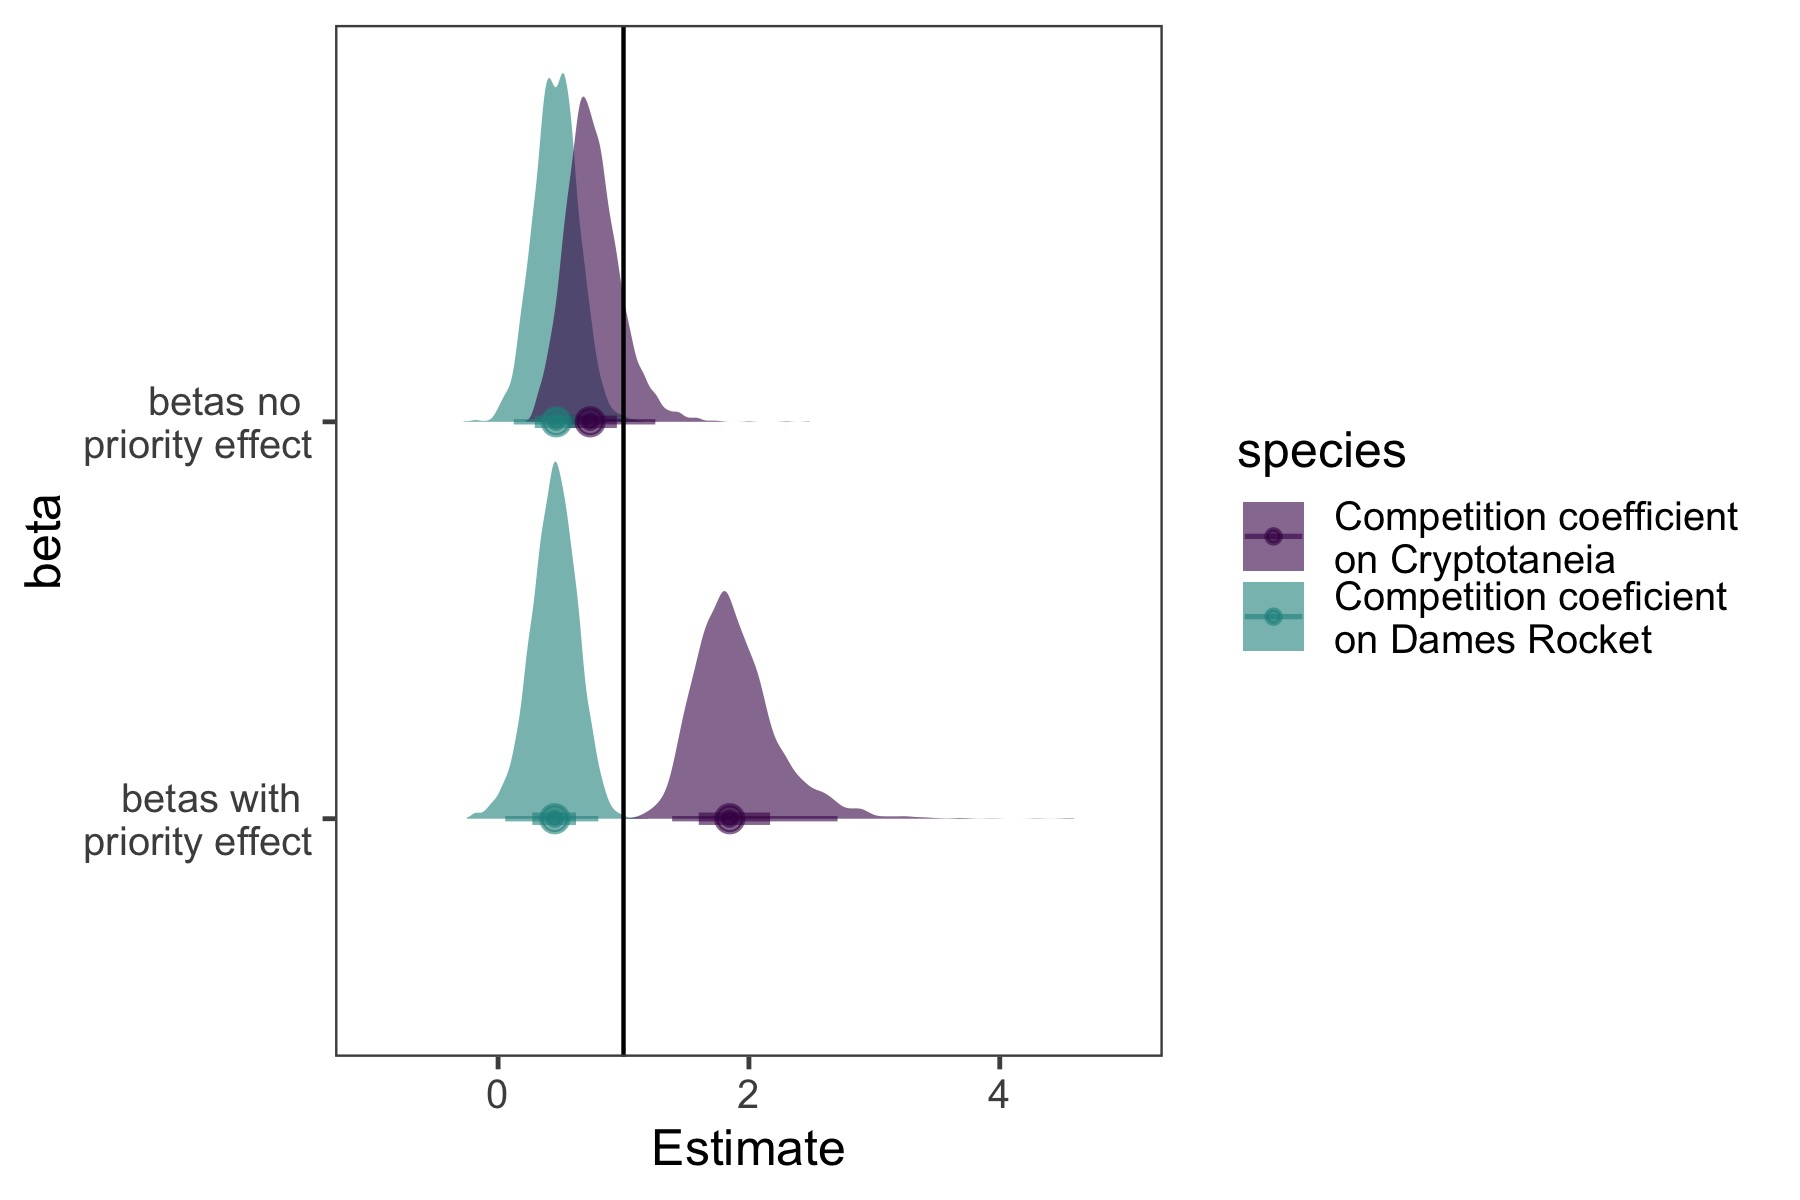
\includegraphics[width=\textwidth]{..//figure/comp_coefficient.jpeg}
    \caption{Estimated of competition coefficients with and without priority effect. Without priority effect, species would be expected to coexist (for both species, intra-specific competition is highe than interspecific i.e. coefficients are less than one). When just one day of priority effects are included in the calculation Dames rocket's interspecific competition increases realtive to its intraspecific competition strength, suggesting with will ultimately competitively exclude Honewort.  } 
    \label{fig:Cc}
\end{figure}

\begin{figure}[h!]
    \centering
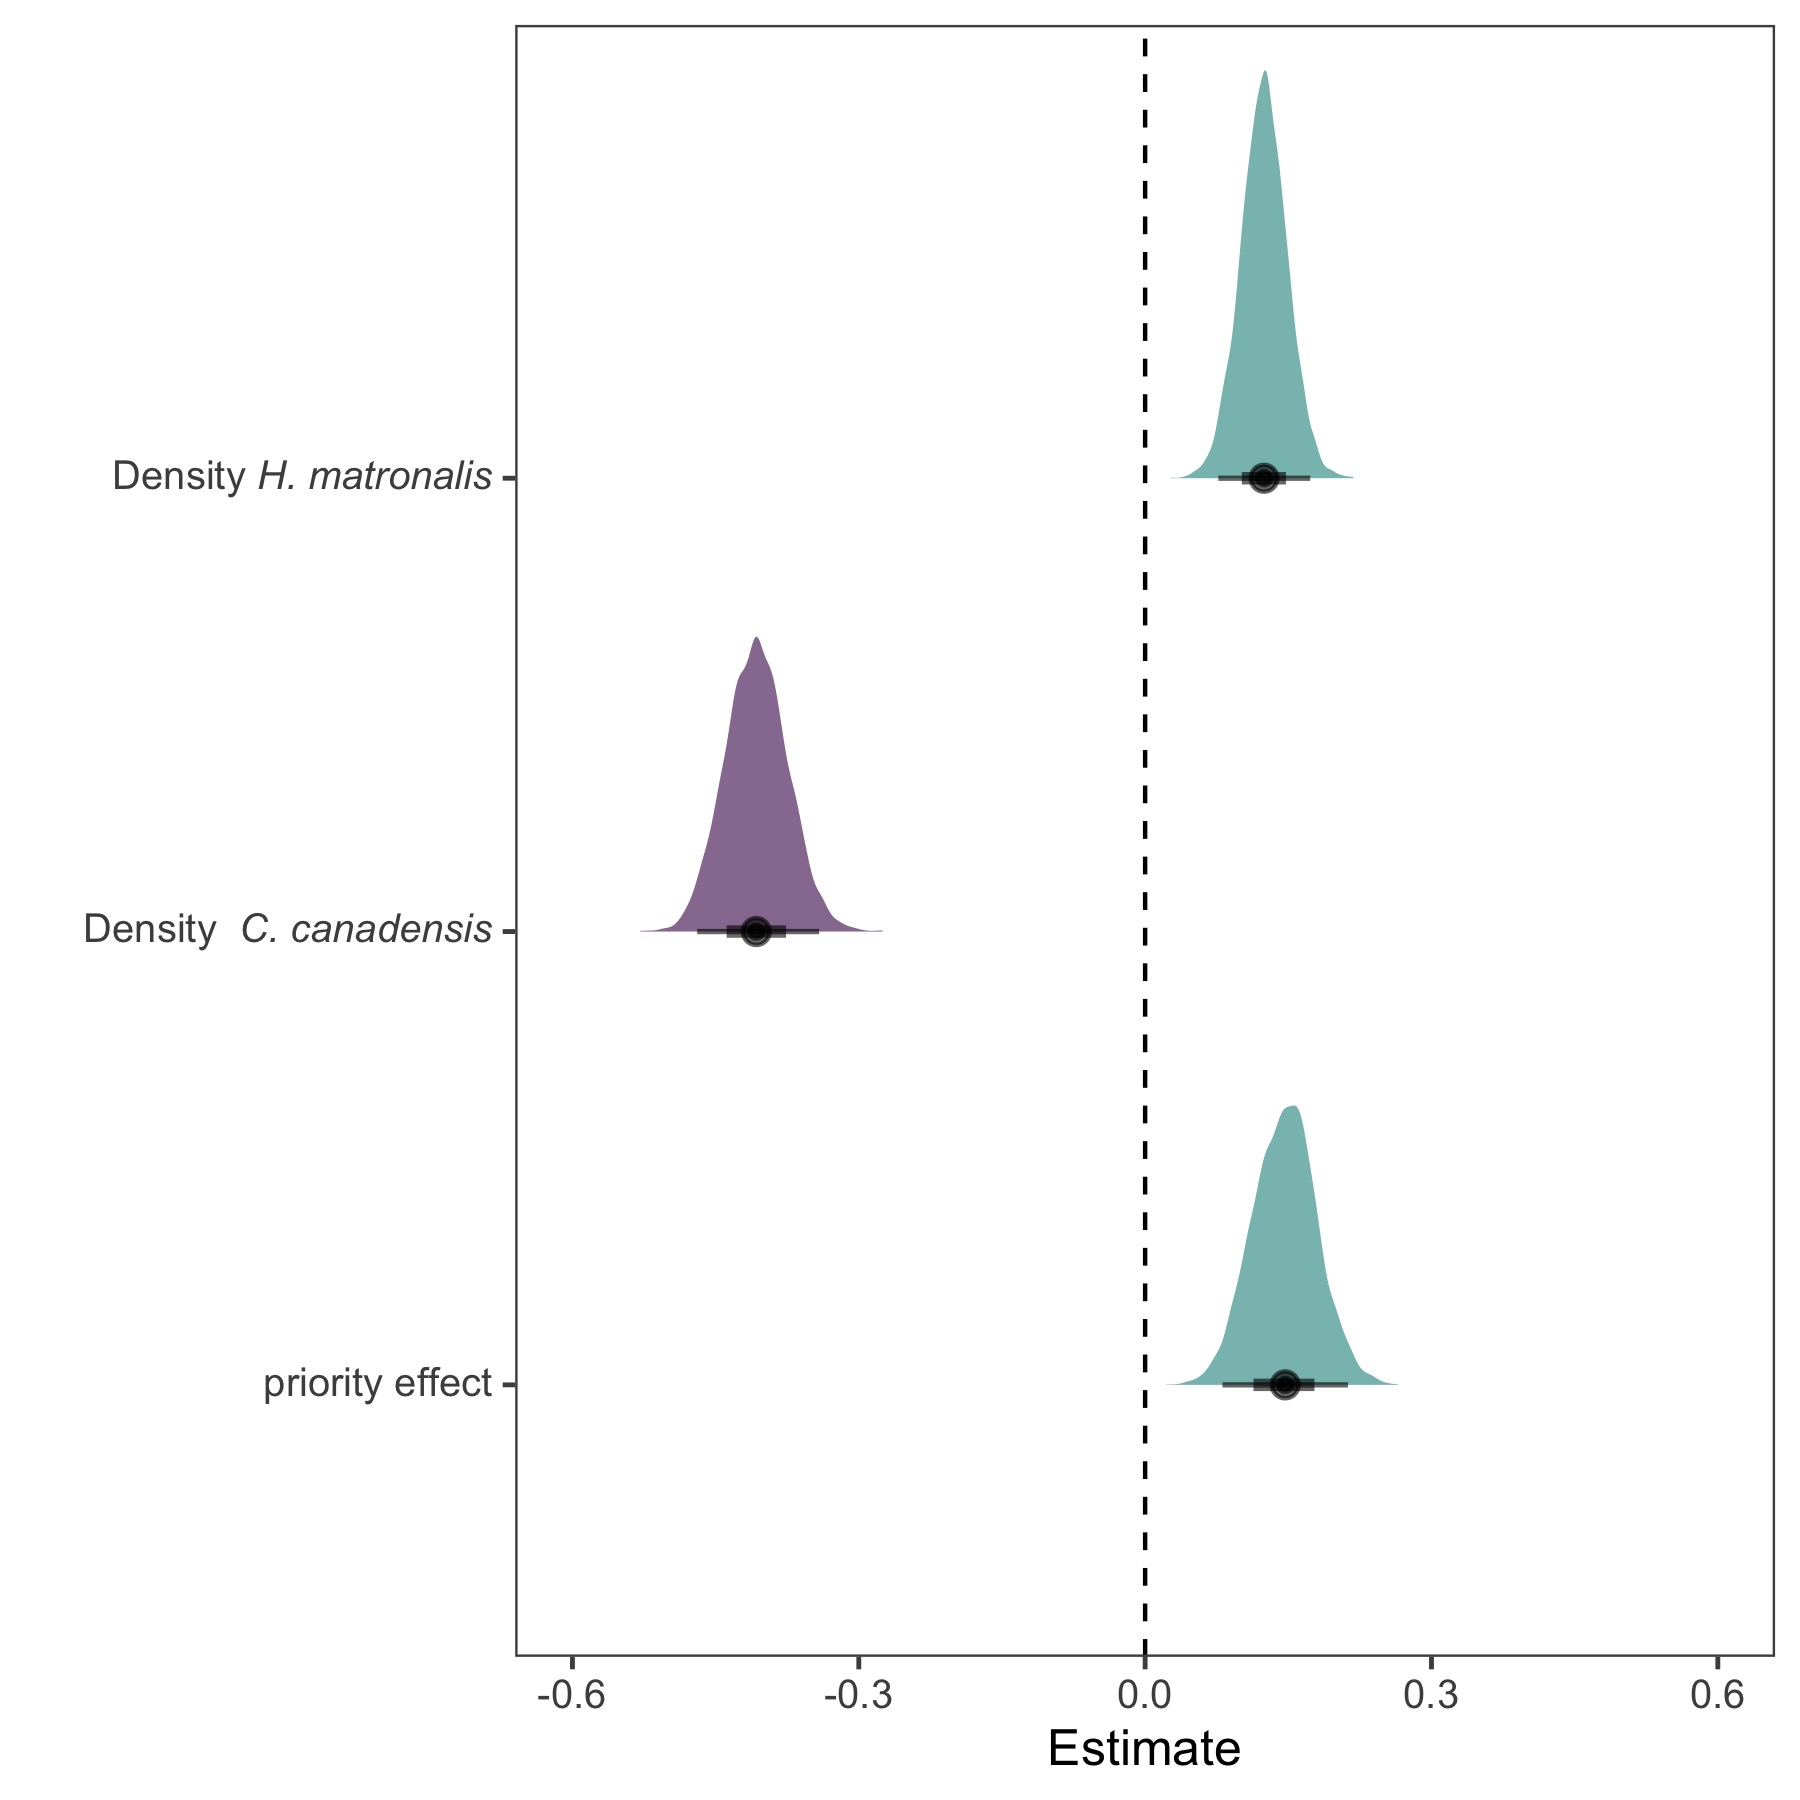
\includegraphics[width=\textwidth]{..//figure/mu_plots.jpeg}
    \caption{Estimated effects of density influence parameters and temporal priority effect on the relative growth rate difference between \textit{H. matronalis} and \texit{C. canadensis}. As per Connonly and Wayne 2005, The positive estimate of priorty and density of Hesperis matronalis tip competitive balance towards it, while the negative estimate of density of C. canadensis favor that species. Like Fig. 2, this suggests that priorty effects are a key mediator of competitive sucess in H. matronalis.  } 
    \label{fig:RGRD}
\end{figure}

\begin{figure}[h!]
    \centering
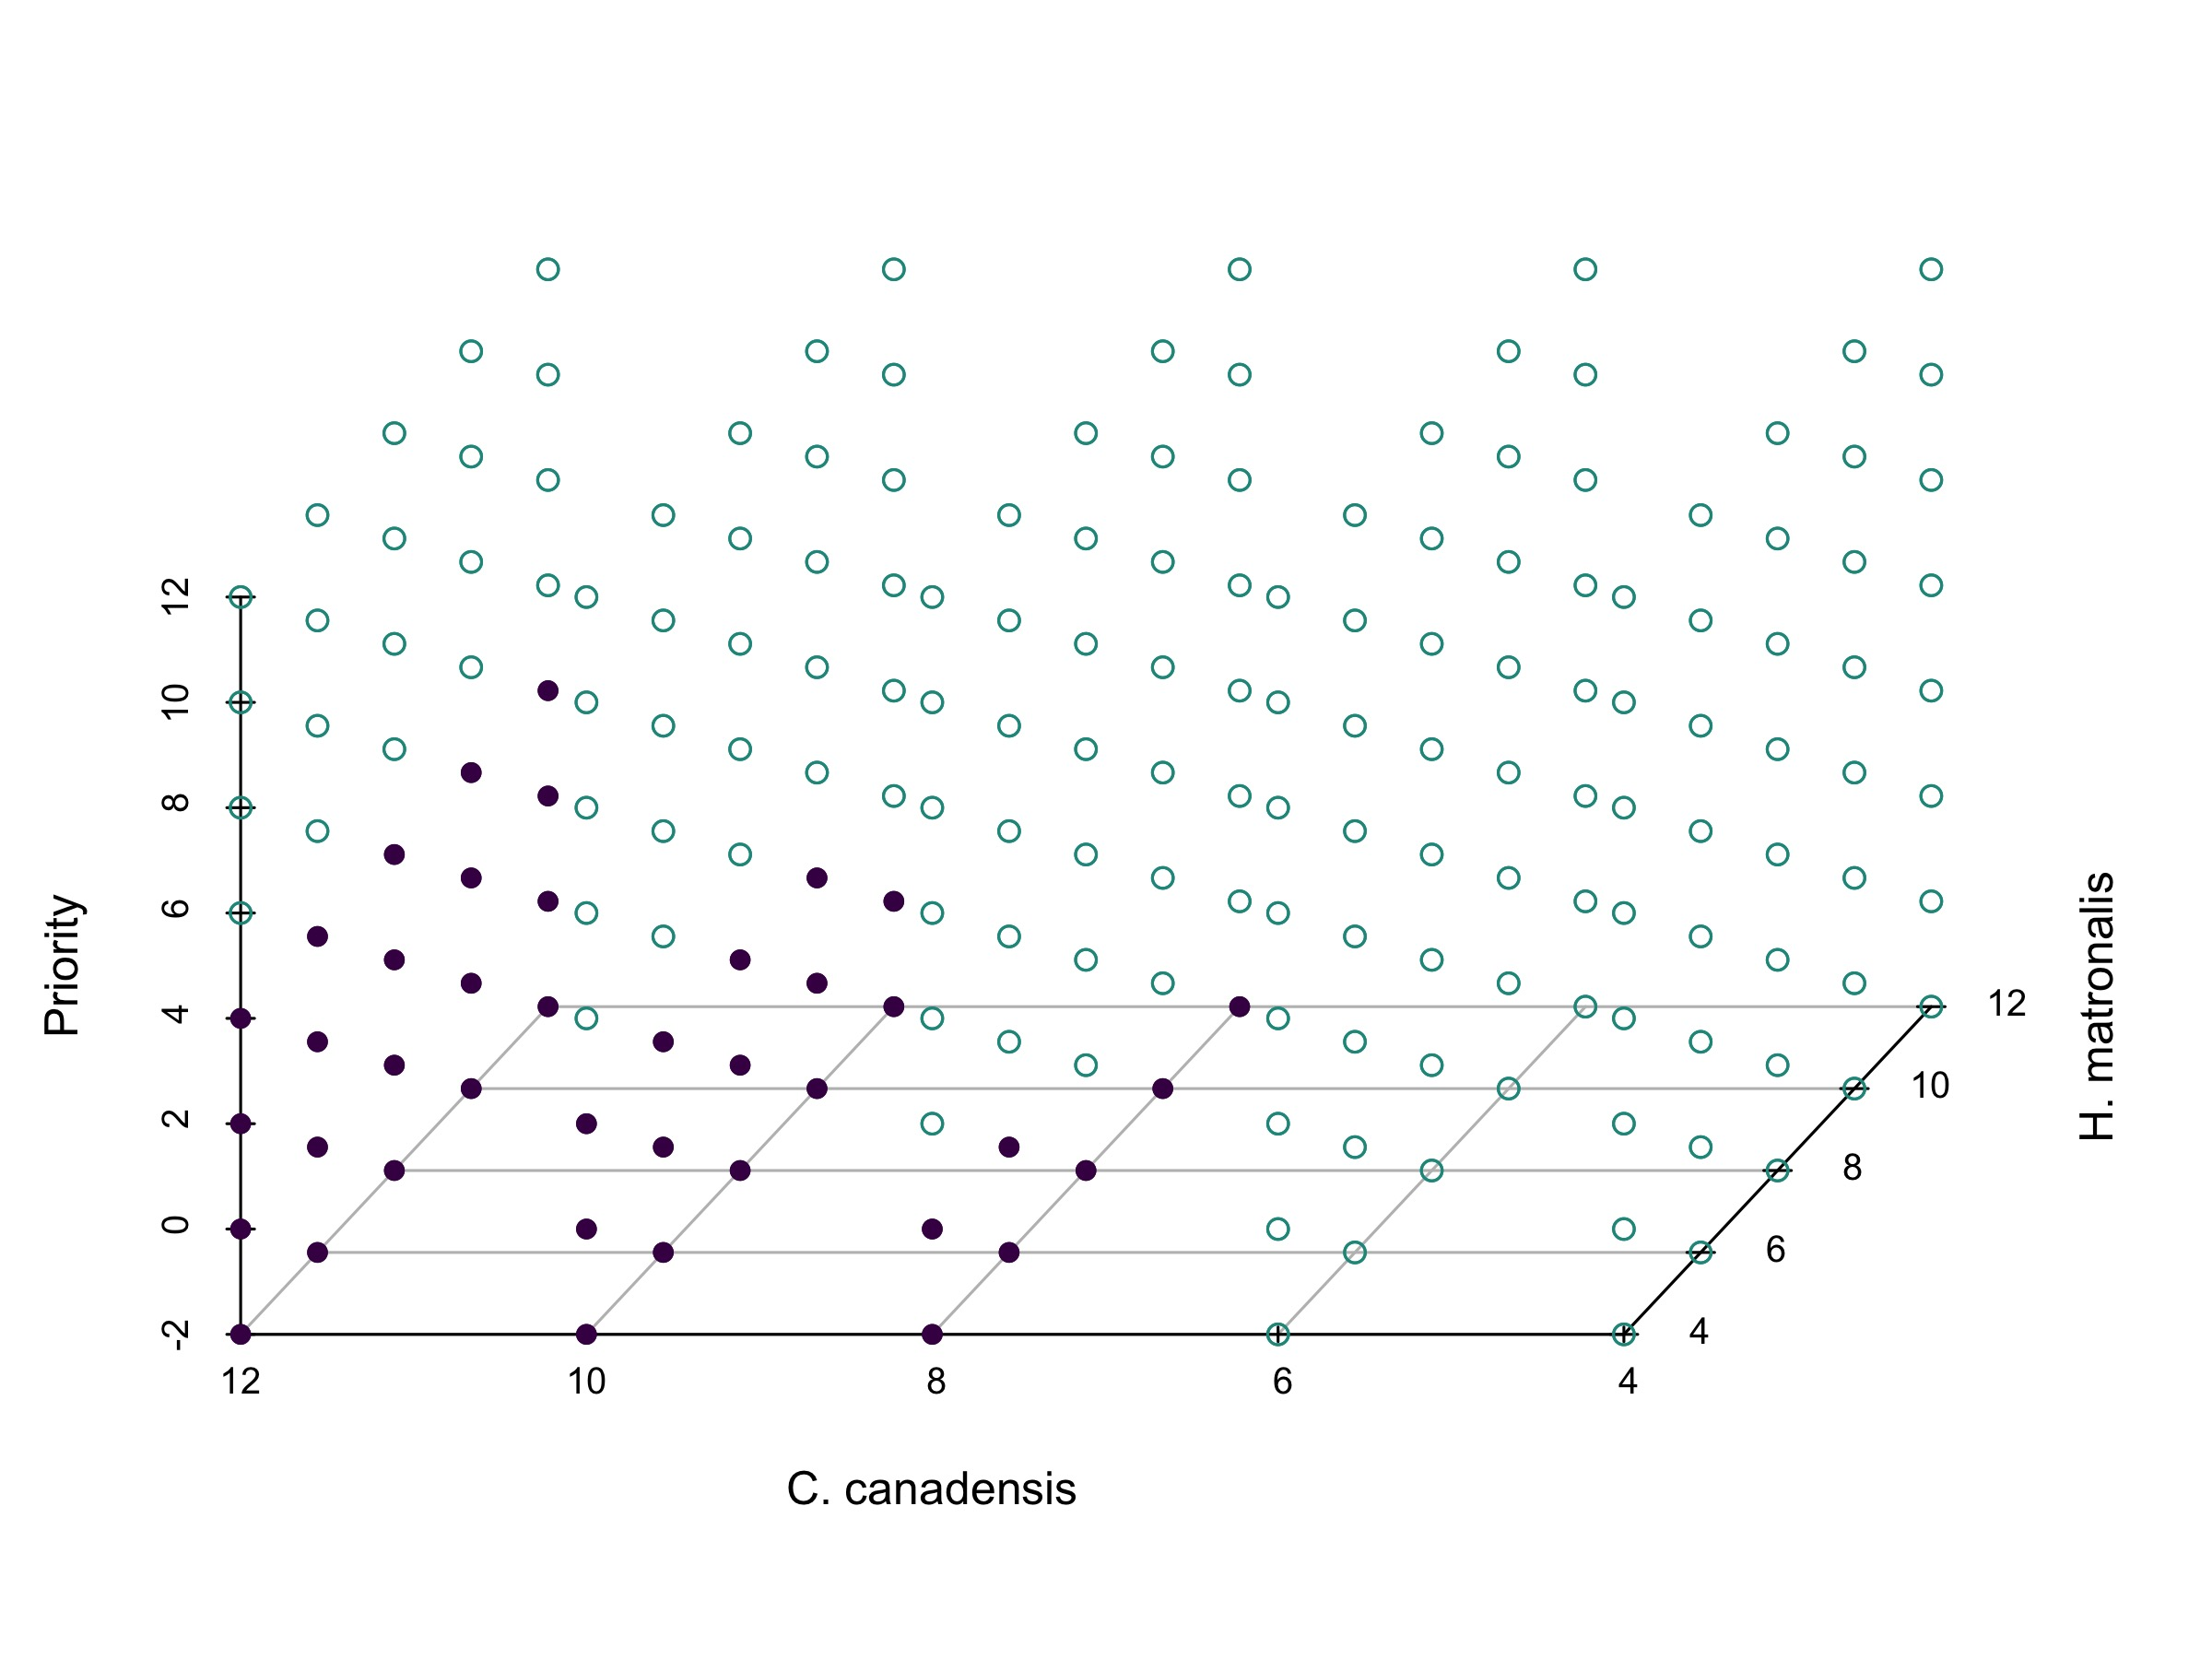
\includegraphics[width=\textwidth]{..//figure/threedpred.jpeg}
    \caption{Predicted outcome of competition under vary inter-specific densities and temporal priority. Purple is \texit{C. canadensis} and green \textit{H. matronalis}. Need to add legend here. As can been seen C. canadensis is predicted to compete with H matronalis only at low priority effects or high densities. } 
    \label{fig:Hm}
\end{figure}





\end{document}
